\documentclass[aspectratio=169]{beamer}
\usepackage{ctex}
\usepackage{graphicx}
\usepackage{booktabs}
\usepackage{tikz}

\usetheme{Madrid}
\usecolortheme{seahorse}
\setbeamertemplate{navigation symbols}{}
\setbeamertemplate{footline}{}

\title{智慧课堂助手}
\subtitle{软件工程探索与实践}
\author{颜宇翔 \quad 魏天翼 \quad 蒋天源}
\institute{小组项目汇报}
\date{2026年5月26日}

\begin{document}

% ---- 封面 ----
\begin{frame}
  \titlepage
\end{frame}

% ---- 选题介绍 ----
\begin{frame}{选题介绍}
  \begin{block}{项目背景}
    \begin{itemize}
      \item 在线课堂（雨课堂等）中，学生需要快速理解课件内容
      \item 传统方式：手动截图、记笔记，效率低且容易遗漏
      \item 需求：实时捕获课件、AI 辅助分析、划词翻译
    \end{itemize}
  \end{block}

  \begin{block}{项目目标}
    \begin{itemize}
      \item 自动捕获课堂课件图片（在线/离线模式）
      \item AI 智能解析：分类、要点提炼、题目解答
      \item OCR 精确文字层 + 划词翻译/解释
      \item 深度思考：对课件内容做深入分析
    \end{itemize}
  \end{block}
\end{frame}

% ---- 技术方案：总体架构 ----
\begin{frame}{技术方案 —— 总体架构}
  \begin{columns}[T]
    \begin{column}{0.48\textwidth}
      \begin{block}{前端（Electron 桌面端）}
        \begin{itemize}
          \item Electron + BrowserView 内嵌雨课堂
          \item PDF.js 渲染离线 PDF 文档
          \item KaTeX + marked.js 渲染公式与 Markdown
          \item OCR 文字层覆盖，支持划词选择
        \end{itemize}
      \end{block}
    \end{column}
    \begin{column}{0.48\textwidth}
      \begin{block}{后端（Node.js 服务）}
        \begin{itemize}
          \item Express RESTful API + SSE 推送
          \item OpenAI 兼容接口（多模型路由）
          \item Tesseract.js OCR（中英双语 WASM）
          \item SHA-1 图像哈希去重
          \item 流式响应：翻译、聊天、深度分析
        \end{itemize}
      \end{block}
    \end{column}
  \end{columns}

  \vspace{0.4cm}
  \begin{block}{整体流程}
    课件图片捕获 $\rightarrow$ 哈希去重/尺寸过滤 $\rightarrow$ AI 视觉分析 $\rightarrow$ OCR 文字层 $\rightarrow$ 前端展示
  \end{block}
\end{frame}

% ---- 技术方案：在线课件捕获 ----
\begin{frame}{技术方案 —— 在线课件捕获}
  \begin{block}{Chrome DevTools Protocol (CDP) 网络拦截}
    \begin{itemize}
      \item 通过 \texttt{webContents.debugger.attach('1.3')} 附加 CDP 调试器
      \item 监听 \texttt{Network.responseReceived} 筛选 \texttt{image/*} 类型响应
      \item 在 \texttt{Network.loadingFinished} 时调用 \texttt{getResponseBody} 获取完整图片
    \end{itemize}
  \end{block}

  \begin{block}{可见图片扫描（兜底机制）}
    \begin{itemize}
      \item 每 2.5 秒通过 \texttt{executeJavaScript} 扫描 DOM 中大面积 \texttt{<img>}
      \item 按面积排序取前 8 张，补充 CDP 未捕获的资源
    \end{itemize}
  \end{block}

  \begin{block}{课堂状态智能判断}
    \begin{itemize}
      \item URL 正则匹配 + 页面标题关键词检测（课堂/签到/答题）
      \item 据此决定是否激活图片捕获管线
    \end{itemize}
  \end{block}
\end{frame}

% ---- 技术方案：图像去重与过滤 ----
\begin{frame}{技术方案 —— 图像去重与过滤}
  \begin{block}{三级去重策略}
    \begin{enumerate}
      \item \textbf{URL 级去重}：维护 \texttt{interceptedUrls: Set}（上限 500，LRU 淘汰）
      \item \textbf{SHA-1 内容哈希}：对图片 buffer 计算哈希，\texttt{seenHashes: Map} 记录已见图片
      \item \textbf{连续帧防抖}：\texttt{lastSubmittedHash} 过滤视频流重复帧
    \end{enumerate}
  \end{block}

  \begin{block}{尺寸与宽高比过滤}
    \begin{itemize}
      \item 使用 \texttt{sharp} 读取元数据，过滤过小图片（$<$ 阈值宽高）
      \item 过滤宽高比异常（$>6$ 或 $<0.3$）的 UI 元素图片
    \end{itemize}
  \end{block}
\end{frame}

% ---- 技术方案：AI 智能分析 ----
\begin{frame}{技术方案 —— AI 智能分析}
  \begin{block}{多模态视觉分析}
    \begin{itemize}
      \item 图片转 \texttt{data:image/...;base64,...} 以 \texttt{image\_url} 发送
      \item System Prompt 要求输出结构化 JSON（分类、要点、解答、OCR 文字）
      \item 五分类体系：课件 / 选择题 / 填空题 / 主观题 / 非课程内容
    \end{itemize}
  \end{block}

  \begin{block}{多模型策略}
    \begin{itemize}
      \item 快速模型（GPT-5.4-mini）：实时解析、翻译
      \item 深度模型（GPT-5.4）：深入分析与拓展
      \item 多端点路由：支持 OpenAI / DeepSeek / GLM 等兼容接口
    \end{itemize}
  \end{block}

  \begin{block}{容错 JSON 解析}
    \begin{itemize}
      \item 修复尾逗号、未转义换行等 LLM 输出畸形问题
      \item 流式 SSE 逐行拼接完整响应后解析
    \end{itemize}
  \end{block}
\end{frame}

% ---- 技术方案：OCR 与划词翻译 ----
\begin{frame}{技术方案 —— OCR 与划词翻译}
  \begin{block}{Tesseract.js OCR 引擎}
    \begin{itemize}
      \item WASM 离线识别，加载 \texttt{chi\_sim+eng} 双语言模型
      \item TSV 结构化输出：解析 level=5（词级）获取每词 \texttt{\{text, x, y, w, h\}}
      \item 单例 Worker 复用 + 本地模型文件缓存
    \end{itemize}
  \end{block}

  \begin{block}{划词翻译/解释}
    \begin{itemize}
      \item 三种触发模式：弹出工具栏 / 直接翻译 / 关闭
      \item 词典式结构化翻译：单词返回音标+词性+例句，句子返回整体翻译+关键词汇
      \item SSE 流式实时展示，弹窗支持拖拽定位与 Pin 固定
    \end{itemize}
  \end{block}
\end{frame}

% ---- 技术方案：深度思考与对话 ----
\begin{frame}{技术方案 —— 深度思考与 AI 对话}
  \begin{block}{深度思考}
    \begin{itemize}
      \item 基于基础解析的二次深度分析（原始图片 + 首次解析作为上下文）
      \item 学术结构化输出：核心概念 / 推导原理 / 关联知识 / 典型考题 / 常见误区
      \item 异步状态机管理（thinking → done/error），前端 SSE 实时更新
    \end{itemize}
  \end{block}

  \begin{block}{AI 对话}
    \begin{itemize}
      \item 结合当前课件图片上下文的智能问答
      \item 流式响应实时展示，支持多轮对话
      \item Markdown + KaTeX 实时渲染回答内容
    \end{itemize}
  \end{block}
\end{frame}

% ---- 技术方案：离线模式 ----
\begin{frame}{技术方案 —— 离线 PDF 模式}
  \begin{block}{PDF.js 客户端渲染}
    \begin{itemize}
      \item PDF.js 3.11 解析 PDF，\texttt{page.render()} 渲染到 Canvas
      \item 支持 \texttt{devicePixelRatio} 高清缩放
    \end{itemize}
  \end{block}

  \begin{block}{性能优化}
    \begin{itemize}
      \item \texttt{IntersectionObserver}（rootMargin: 200px）懒加载
      \item 仅渲染进入视口附近的页面，避免一次性渲染数百页
    \end{itemize}
  \end{block}

  \begin{block}{透明文本层}
    \begin{itemize}
      \item \texttt{page.getTextContent()} 获取文字内容及 transform 矩阵
      \item 绝对定位 \texttt{<span>} 叠加在 Canvas 上方（透明不可见）
      \item 支持原生文本选中 → 触发划词翻译
    \end{itemize}
  \end{block}
\end{frame}

% ---- 功能演示 ----
\begin{frame}{功能演示（一）}
  \begin{center}
    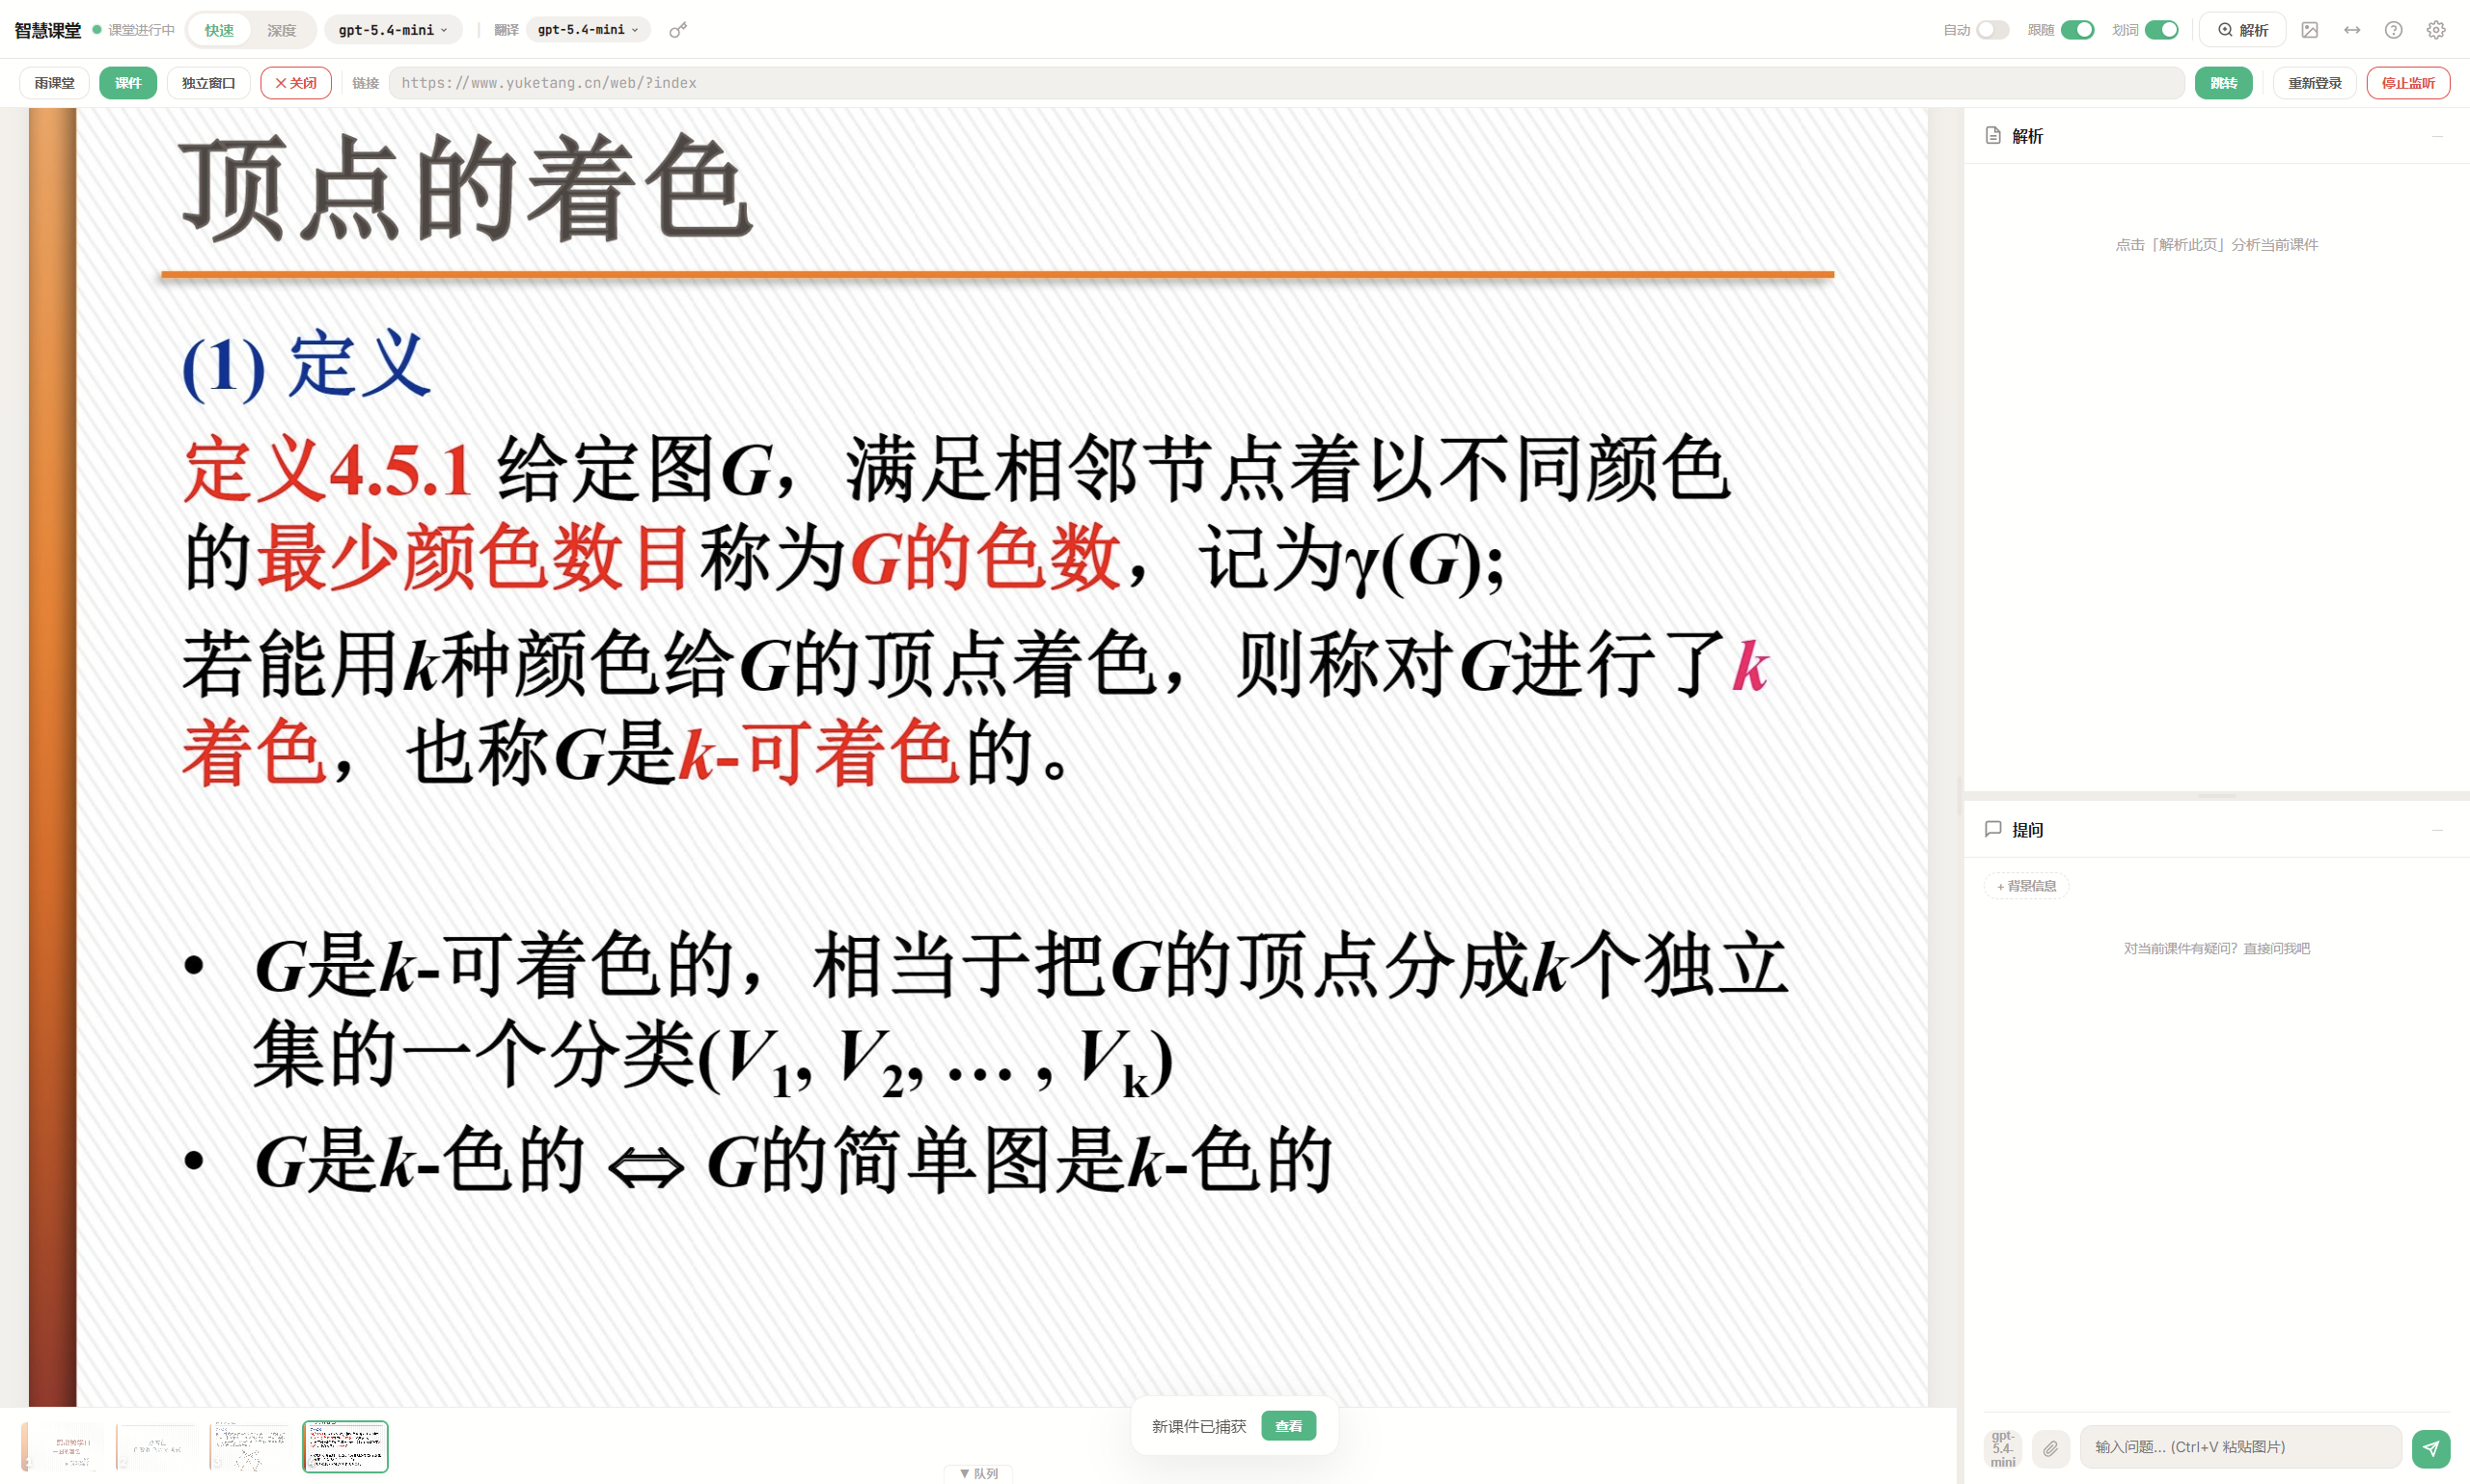
\includegraphics[width=0.85\textwidth]{demo1.png}
  \end{center}
\end{frame}

\begin{frame}{功能演示（二）}
  \begin{center}
    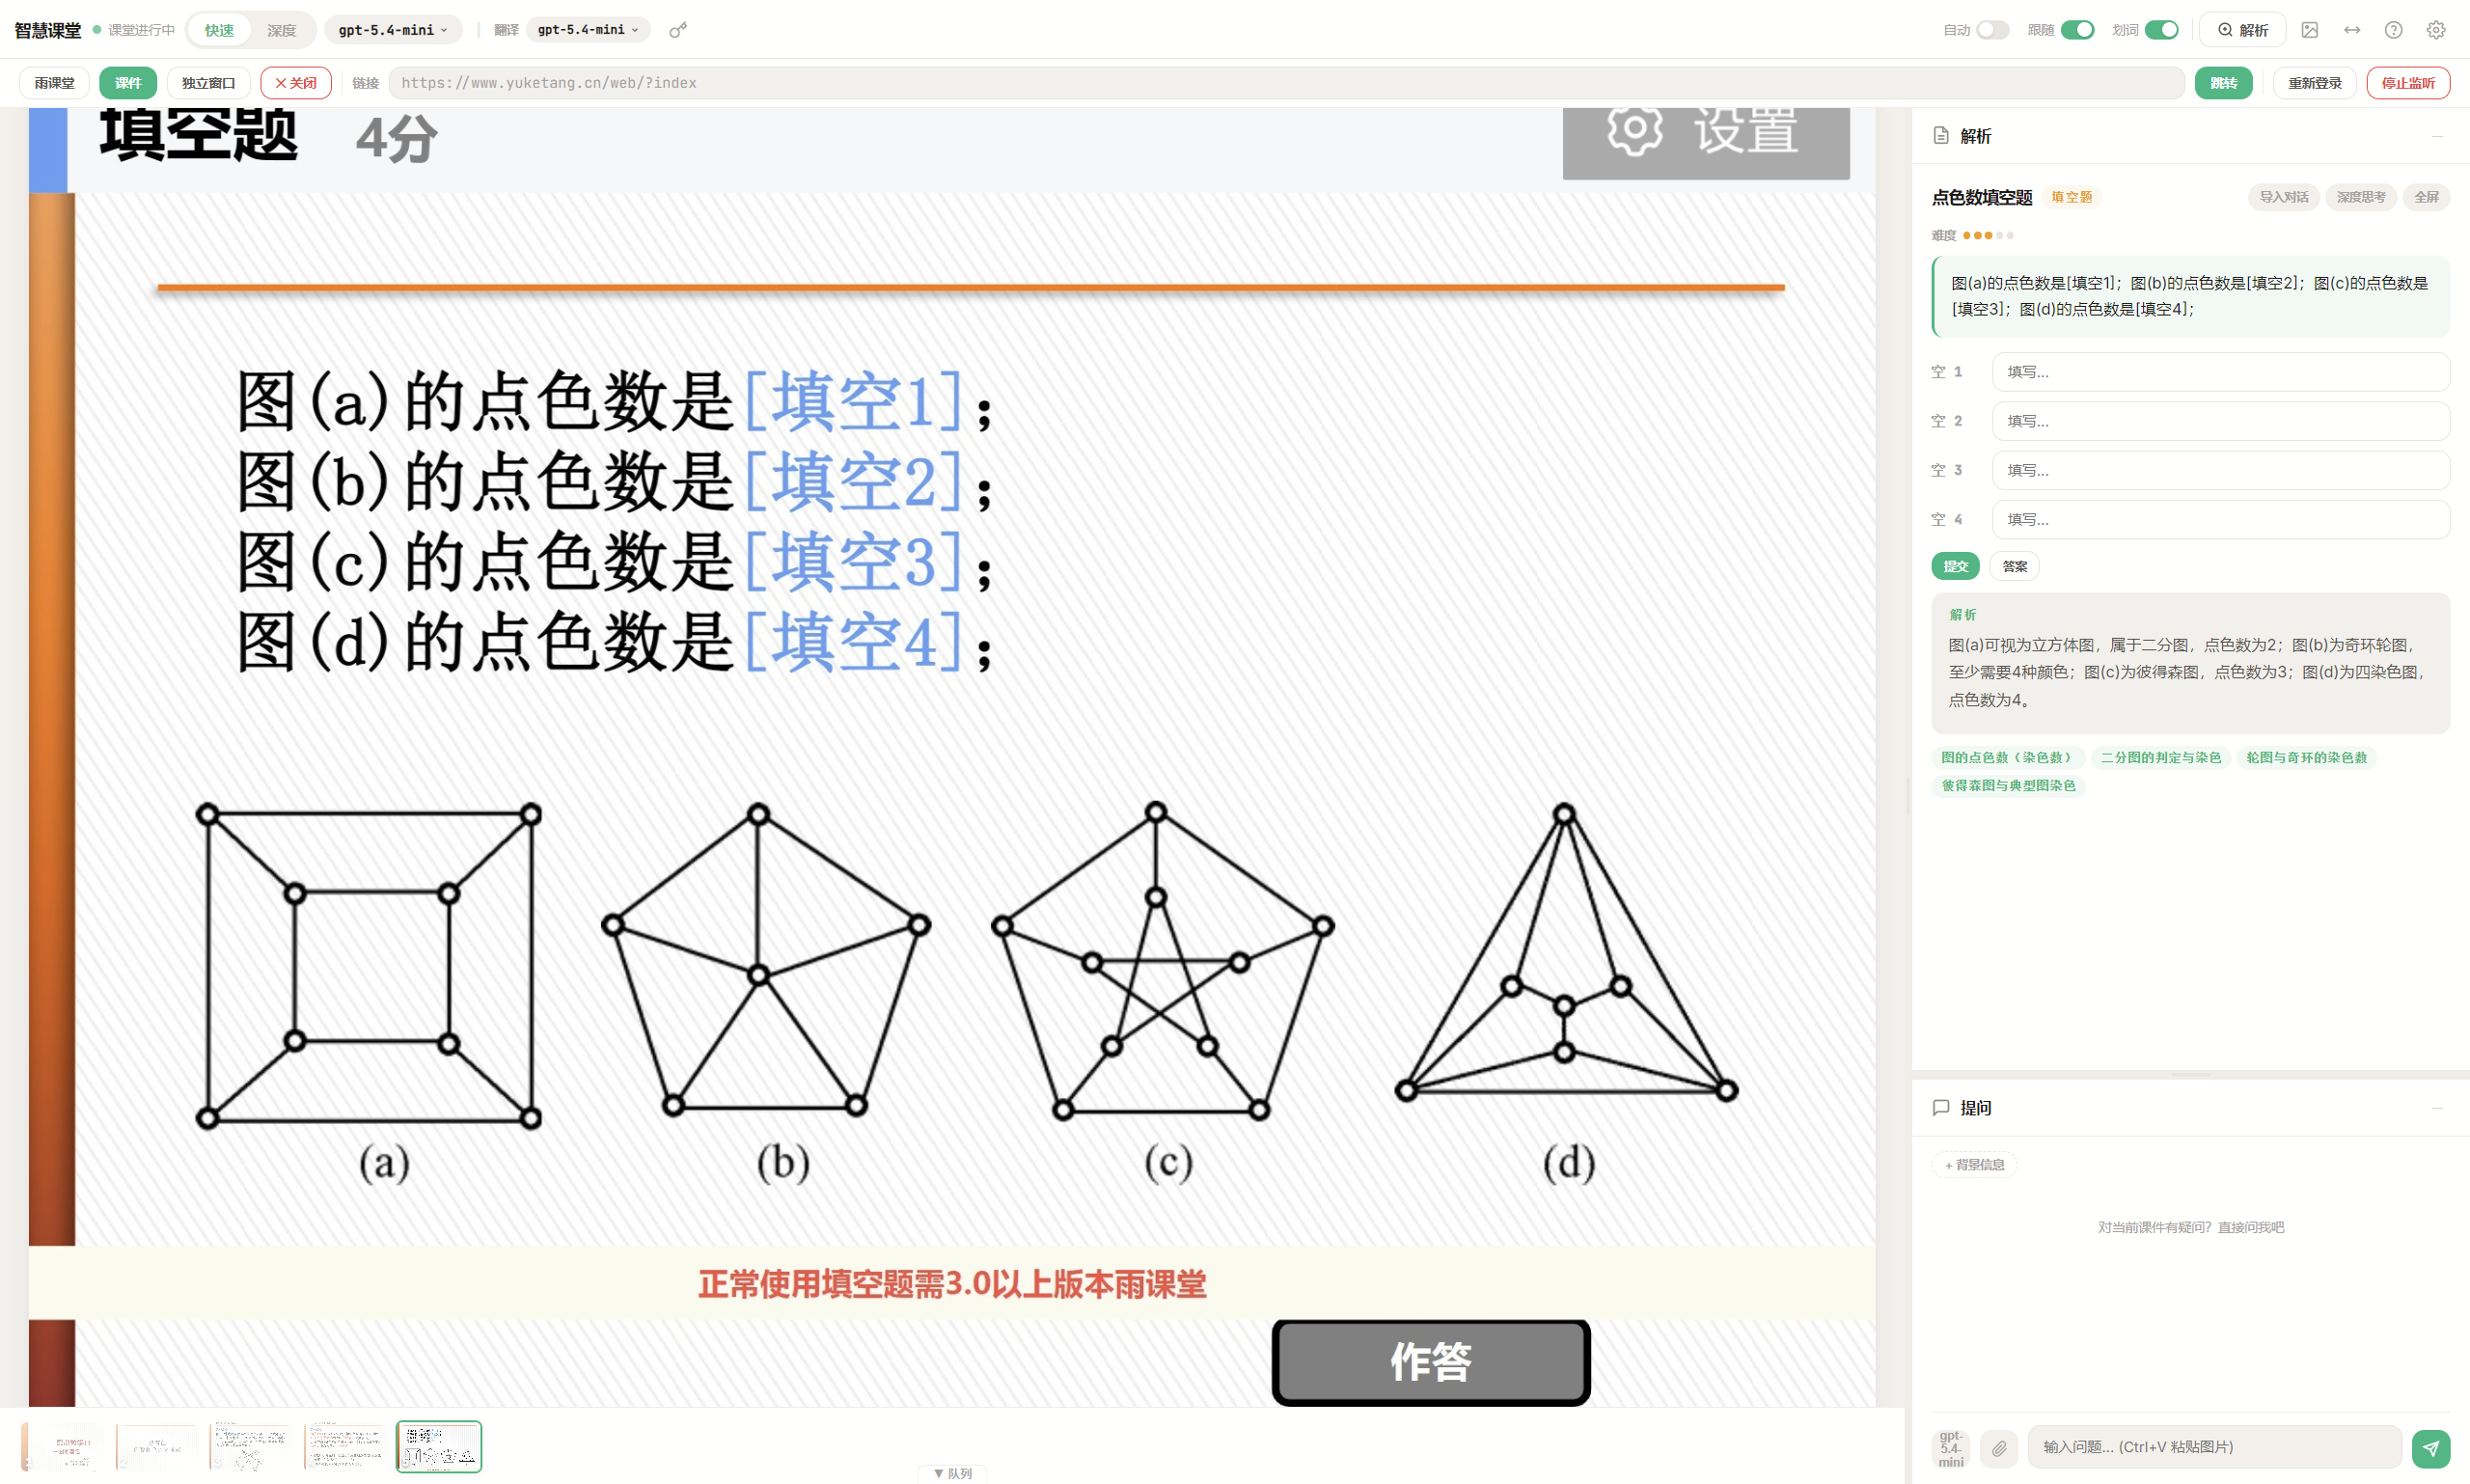
\includegraphics[width=0.85\textwidth]{demo2.png}
  \end{center}
\end{frame}

\begin{frame}{功能演示（三）}
  \begin{center}
    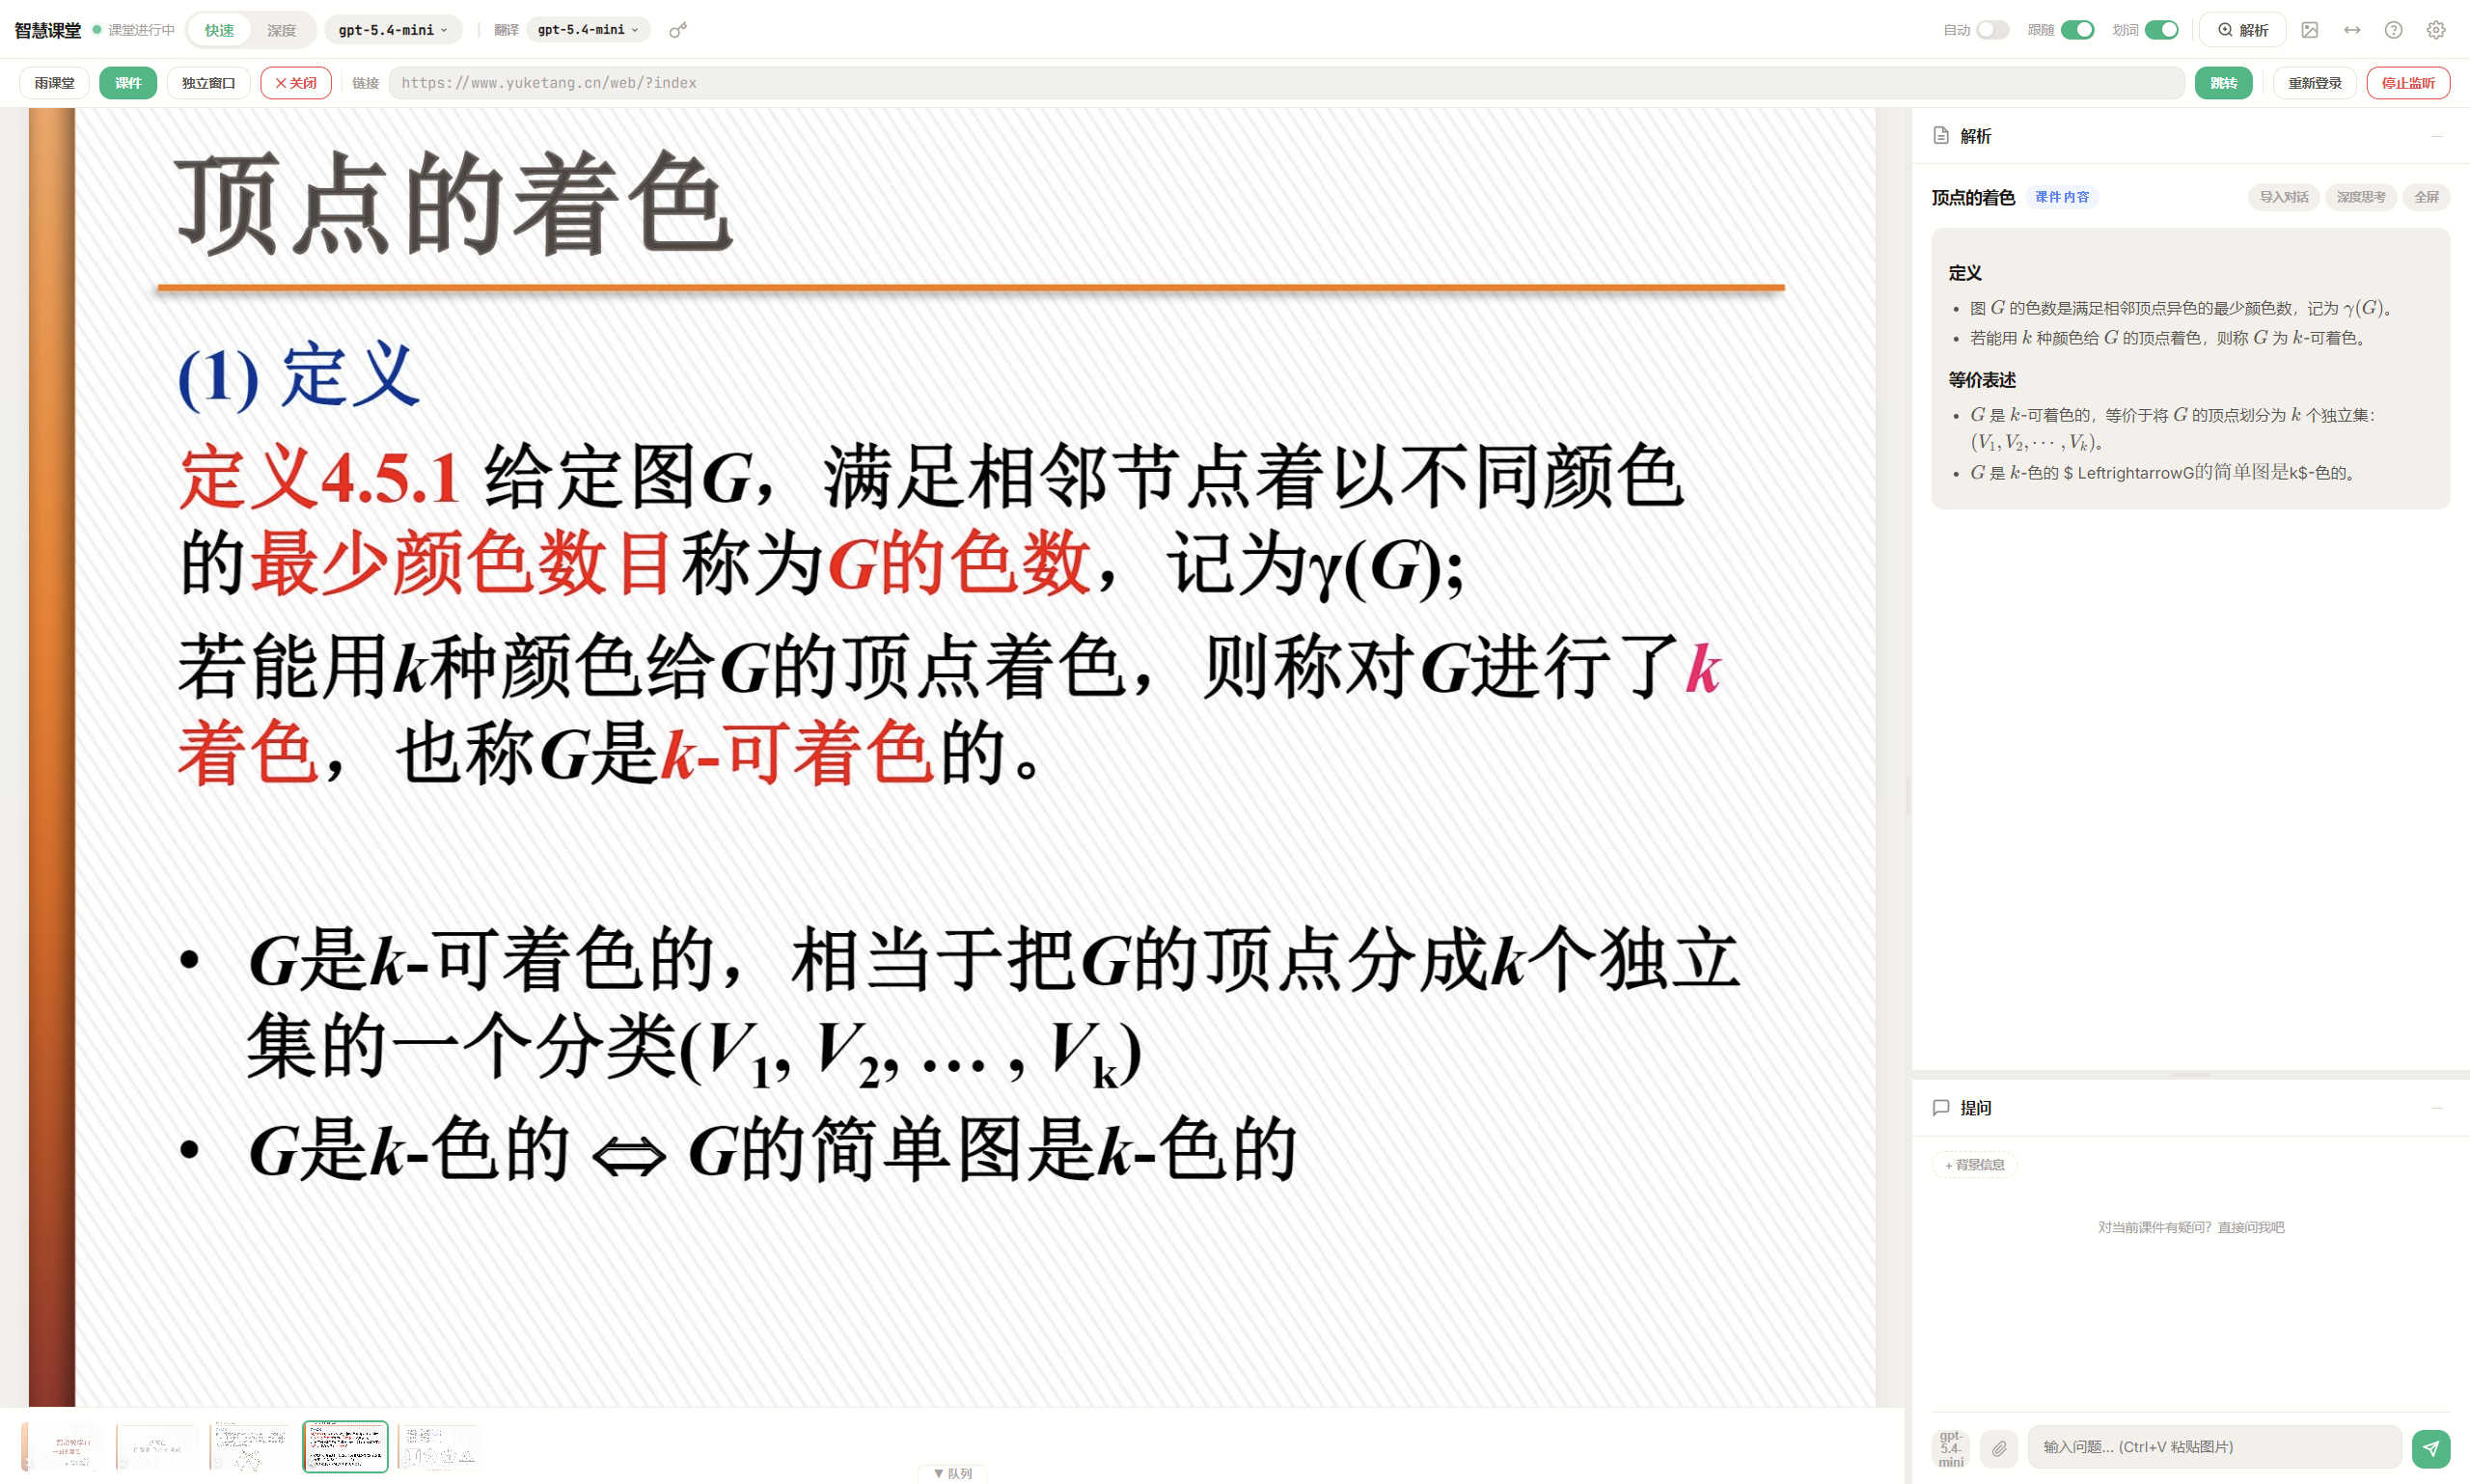
\includegraphics[width=0.85\textwidth]{demo3.png}
  \end{center}
\end{frame}

% ---- 团队分工 ----
\begin{frame}{团队分工}
  \begin{table}[h]
    \centering
    \renewcommand{\arraystretch}{1.5}
    \begin{tabular}{lll}
      \toprule
      \textbf{成员} &  \textbf{主要职责} \\
      \midrule
      颜宇翔 & 前端界面开发、交互设计与 OCR 集成  \\
      魏天翼 & 后端服务开发、AI 接口对接与流式通信  \\
      蒋天源 & Electron 主进程、CDP 课件捕获与打包部署  \\
      \bottomrule
    \end{tabular}
  \end{table}

  \vspace{0.5cm}
  \begin{block}{协作方式}
    \begin{itemize}
      \item Git 版本管理，多分支协作
      \item 统一 RESTful API 接口规范
      \item 迭代开发，持续集成
    \end{itemize}
  \end{block}
\end{frame}

% ---- 后续规划 ----
\begin{frame}{后续规划}
  \begin{enumerate}
    \item \textbf{集成 RAG}：引入检索增强生成，结合课件知识库提升 AI 回答准确性
    \item \textbf{更可视化便捷的知识库管理}：提供图形化界面管理课件资料、笔记与历史记录
    \item \textbf{AI 辅助笔记系统}：类似 Notion 的块编辑器，支持 AI 自动总结、补全与整理
    \item \textbf{优化交互体验和便捷程度}：简化操作流程，提升响应速度与界面友好度
  \end{enumerate}
\end{frame}

% ---- 结尾 ----
\begin{frame}
  \centering
  \vspace{2cm}
  {\Huge 谢谢！}
\end{frame}

\end{document}
